


\section{Synthèse et dépôt de la couche d'ITO}

\subsection{Protocole de dépôt par Dip-Coating}

\begin{enumerate}
\item Préparation de la solution (Sol) : Une solution d'ITO à \SI{10}{\percent} en masse d'étain a été préparée par le technicien et pourra être utilisée dans ce TP.

\item Procédure de Dépôt par Dip-Coating :
\begin{enumerate}
\item Préparation des substrats : Nettoyer les plaques de verre à l'eau distillée, à l'éthanol, puis sécher à l'air.  %- Éventuellement, traiter par plasma pour améliorer l’adhérence.
\item Dépôt du film : 
\begin{enumerate}
\item Préparer un bécher de \SI{25}{\milli\liter} contenant le sol ;
\item Règler le dip coater à une vitesse d'immersion de \SI{10}{\centi\meter\per\minute}, un temps de séjour de \SI{1}{\minute}.
\item Récupérer vos plaques de verre et laisser les sécher à l'air libre
\end{enumerate}

\item Traitement thermique (recuit) : Chauffer les échantillons à \SI{650}{\celsius} pendant \SI{30}{\minute} dans l'air dans un des fours à moufle.

Pour obtenir des films plus épais ($~ \sim 200$-\SI{300}{\nano\meter}), répéter le cycle dépôt-séchage-recuit plusieurs fois. 

Une autre étude a montré l'influence du temps de recuit sur la transmittance de la plaque d'ITO.

\begin{center}
\begin{minipage}{0.48\textwidth}
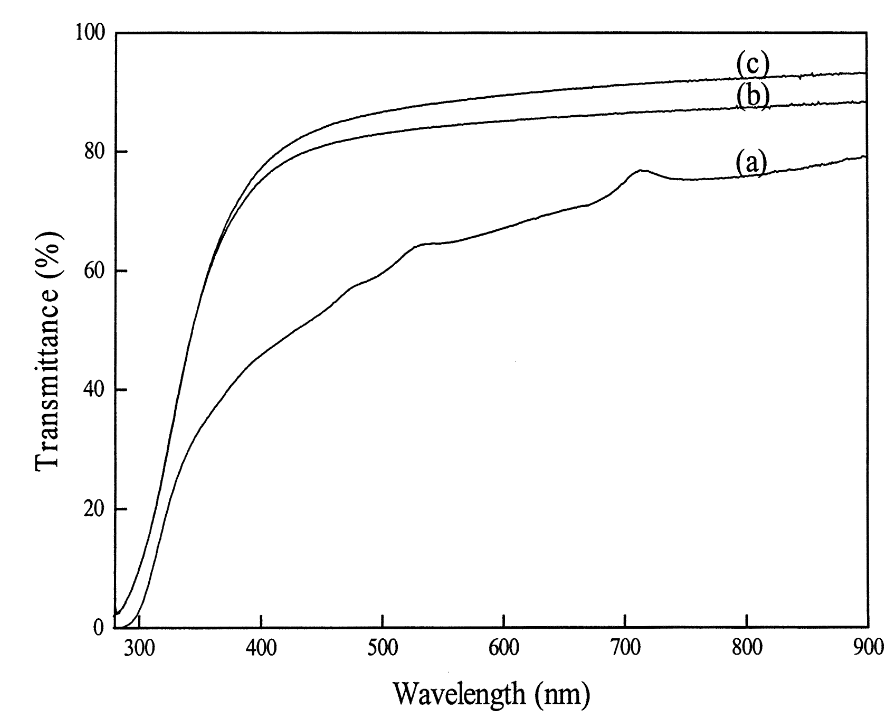
\includegraphics[width=\textwidth]{figures/Fig05b}
\end{minipage}\begin{minipage}{0.48\textwidth}
\captionof{figure}{Evolution de la transmittance de la plaque d'ITO en fonction de la longueur d'onde pour des couches de \SI{250}{\nano\meter} d'épaisser et une température de recuit de \SI{400}{\celsius}, \SI{500}{\celsius} et \SI{600}{\celsius}}
\end{minipage}
\end{center}

\end{enumerate}
\item Caractérisations possibles : ohmmètre, brillancemètre, colorimètre et DRX.
\end{enumerate}

\subsection{Questions sur le dépôt d'ITO}

Les conditions optimales que l'on peut espérer avec cette procédure selon la littérature sont les suivantes : 
\begin{itemize}
\item Résistivité optimale : $\rho = 1.7 \cdot 10^{-3} ~ \si{\ohm\centi\meter}$ ;
\item Transmittance dans le visible : $> 90 ~ \si{\percent}$
\end{itemize}

\begin{questions}
\setcounter{question}{\thefoo}
\question[2] Quelle est l'influence de la vitesse d'immersion du dip-coater sur l'épaisseur de la couche déposée ?

\begin{mybox}
\begin{solution}[5cm]

\textbf{Relation de Landau-Levich} [\textbf{1.0}] Pour de faibles vitesse et des effets capillaires dominant devant le poids, l'épaisseur vaut :

\begin{align*}
e \propto \frac{(\eta V)^{2/3}}{\gamma^{1/6} \rho g}
\end{align*}

avec $\gamma$ le coefficient de tension de surface,  $\rho$ la masse volumique du fluide, $g$ le champ de pesanteur, $\eta$ la c{\oe}fficient de tension de surface et $V$ la vitesse de sortie de la plaque du fluide.

\textbf{Interprétation} [\textbf{1.0}] A priori, plus la vitesse de sortie de la plaquée est elevée et plus l'épaisseur de liquide est élevée.

\end{solution}
\end{mybox}

Dans des conditions opératoires similaires aux nôtres, une équipe de chercheur a établi un lien entre la taille des cristallites du sol, la température de recuit et la résistivité du milieu : 
\begin{center}
\begin{minipage}{0.46\textwidth}
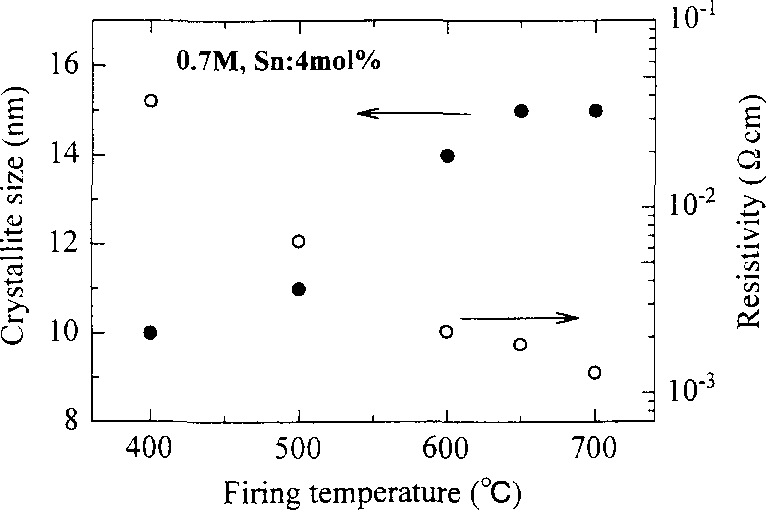
\includegraphics[width=\textwidth]{figures/Fig05}
\end{minipage}\hfill\begin{minipage}{0.46\textwidth}
\captionof{figure}{Relation entre la taille des cristallites, la conductivité et la température de recuit pour un sol de concentration \SI{0.7}{\mole\per\liter}, 2 cycles dépôt-séchage-recuit et une vitesse d'immersion \SI{6}{\centi\meter\per\minute}}
\end{minipage}
\end{center}

\question[3] D'après ce graphe, que peut-on dire des conditions de recuit utilisées ? Quelle relation structure-propriété peut-on établir ?

\begin{mybox}
\begin{solution}[5cm]

\textbf{Influence sur la taille :} [\textbf{1.0}] Formation de cristaux de grande taille ($\approx 15 ~ \si{\nano\meter}$)

\textbf{Influence sur la résistivité :} [\textbf{1.0}] permet d'arriver à des valeurs conformes avec un bon semi-conducteur $\sigma \sim 10^3 ~ \si{\siemens\per\centi\meter}$

\textbf{Relation structure-propriété :} [\textbf{1.0}] Taille de grain importante est corrélée à une bonne conductivité, ce qui est conforme avec la diminution de la densité volumique de joints de grain, source de déperdition d'énergie.

\end{solution}
\end{mybox}

\question[2] Mesurer l'évolution des paramètres en fonction du nombre de cycles dépôt-séchage-recuit. Commenter les évolutions observées.

\begin{mybox}
\begin{solution}[5cm]

L'augmentation du nombre de couche déposée, consistante avec une augmentation de l'épaisseur d'ITO, se traduit par une augmentation de la résistance du matériau (dépendant aussi de paramètres géométriques de la couche déposée)

\end{solution}
\end{mybox}

\setcounter{foo}{\thequestion}
\end{questions}
